\subsection{Perspectives: Towards a Derivation of the Proton-to-Electron Mass Ratio}
  \label{subsec:perspectives_mass_spectrum}

  The proton-to-electron mass ratio is one of the most precisely measured dimensionless quantities in physics.
  Within the Cosmochrony framework, the purpose of this section is not to derive this
  value from first principles, but to clarify how such a ratio could emerge
  \emph{structurally} from the spectral and topological organization of localized
  solitonic excitations of the projected field \(\chi_{\mathrm{eff}}\).

  The discussion should therefore be understood as a minimal and exploratory spectral ansatz.
  Its aim is to identify the relevant mechanisms, constraints, and scaling relations
  that any successful derivation would have to satisfy, rather than to provide a complete microscopic calculation.

  \subsubsection{Spectral Stability Hypothesis}

    Let \(\chi_{\mathrm{sol}}\) denote a stationary localized configuration arising in
    the projectable regime of the \(\chi\) dynamics.
    Small perturbations \(\delta\chi_{\mathrm{eff}}\) around this background are
    governed, at the coarse-grained level, by a linear stability operator
    \(\mathcal{L}_{\mathrm{sol}}\), defined as the second variation of an effective localization functional.

    Normal modes satisfy the eigenvalue problem
    \begin{equation}
      \mathcal{L}_{\mathrm{sol}} \psi_n = \lambda_n \psi_n .
    \end{equation}

    The eigenvalues \(\lambda_n\) characterize the resistance of the soliton to
    localized deformations.
    They encode intrinsic stiffness scales associated with the internal organization
    of the solitonic configuration.

    \paragraph{Spectral mass scaling.}
      In regimes where an effective wave description applies, the normal modes exhibit
      characteristic oscillation frequencies
      \begin{equation}
        \omega_n = c \sqrt{\lambda_n} .
      \end{equation}

      Identifying the lowest nontrivial frequency with the rest energy of the excitation
      leads to the effective scaling relation
      \begin{equation}
        m_n \;\propto\; \sqrt{\lambda_n}\,\chi_c ,
      \end{equation}
      where \(\chi_c\) denotes a characteristic geometric scale associated with the
      spatial extension of the solitonic configuration in the projected regime.

      This relation does not define a fundamental mass formula.
      It provides a coarse-grained link between spectral stability and inertial mass,
      consistent with the interpretation of mass as integrated resistance to relaxation.

    \paragraph{Dimensional interpretation.}
      The eigenvalues \(\lambda_n\) carry dimensions of inverse length squared,
      reflecting the restoring stiffness of the soliton per unit deformation.
      The scale \(\chi_c\) has dimensions of length and sets the geometric extension over
      which this stiffness is distributed.

      The combination \(\lambda_n \chi_c^2\) therefore defines a characteristic energy scale,
      \begin{equation}
        E_n \sim \lambda_n \chi_c^2 ,
      \end{equation}
      which is identified with a rest energy through the effective relativistic matching \(E = mc^2\) once a spacetime
      description becomes applicable.

      This identification does not invoke a fundamental quantum constant and remains
      valid independently of the emergence of \(\hbar_{\mathrm{eff}}\).

  \subsubsection{Projection Scale and Effective Normalization}

    The fundamental description of the \(\chi\) field is formulated in terms of
    relational relaxation rules rather than a spacetime action with fixed physical units.
    When a continuum approximation applies, an effective action for perturbations
    around a stable soliton may be introduced as a bookkeeping device.

    In this regime, the effective action for perturbations
    \(\delta\chi_{\mathrm{eff}}\) may be written schematically as
    \begin{equation}
      S_{\mathrm{eff}}[\delta\chi]
      =
      \int d^4x \,
      \frac{1}{2}
      \left( \frac{\chi_c}{c} \right)^2
      \left[
        (\partial_t \delta\chi)^2
      -
      c^2 (\nabla \delta\chi)^2
      \right] .
    \end{equation}

    Expressing this action in emergent spacetime coordinates introduces a geometric
    rescaling factor linking \(\chi\)-space and spacetime lengths.
    As a result, the canonical normalization of localized modes involves a quadratic
    scaling factor of the form
    \begin{equation}
      \left( \frac{\chi_c}{\ell_{\mathrm{spacetime}}} \right)^2 ,
    \end{equation}
    which controls the effective normalization of spectral quantities.

    This factor reflects the geometric projection from the relational \(\chi\) structure to emergent spacetime observables.
    It does not represent a fundamental coupling constant.

  \subsubsection{Energy Levels from Spectral Stability}

    The discrete energy levels associated with solitonic excitations follow from the
    spectral properties of the stability operator \(\mathcal{L}_{\mathrm{sol}}\), not
    from canonical quantization.

    For a soliton labeled by \(n\), the gradient contribution to the effective energy scales as
    \begin{equation}
      E_{\mathrm{grad}}^{(n)}
      \sim
      c^2 \lambda_n \mathcal{N}_n ,
    \end{equation}
    where \(\mathcal{N}_n\) denotes a normalization factor determined by the spatial profile of the mode.

    In the spacetime-based description, this energy is identified with the rest-mass energy,
    \begin{equation}
      E_n \equiv m_n c^2 .
    \end{equation}

    The discretization of \(E_n\) arises from topological classification and spectral
    stability, not from postulated quantum operators.
    The role of \(\hbar_{\mathrm{eff}}\) appears only when matching this description to
    quantum observables.

  \subsubsection{Elementary versus Composite Spectral Structures}

    A key distinction must be drawn between elementary and composite solitonic
    excitations.
    Elementary particles, such as leptons, are expected to correspond to topologically
    elementary solitons whose inertial mass is dominated by a single lowest stability
    eigenvalue.

    By contrast, baryonic excitations are composite configurations.
    Their mass reflects the combined contribution of several coupled stability modes
    associated with a bound structure.
    Mass ratios therefore take the schematic form
    \begin{equation}
      \frac{m_{\mathrm{comp}}}{m_{\mathrm{elem}}}
      \;\sim\;
      \frac{\sum_k \sqrt{\lambda^{(\mathrm{comp})}_k}}
      {\sqrt{\lambda^{(\mathrm{elem})}_0}} ,
    \end{equation}
    rather than the ratio of two isolated eigenvalues.

  \subsubsection{Ansatz for the Proton as a Composite Soliton}

    As an exploratory working hypothesis, the proton is modeled as a composite solitonic excitation.
    Specifically:
    \begin{itemize}
      \item the electron corresponds to a topologically elementary soliton with a
      fundamental stability eigenvalue \(\lambda_e\),
      \item the proton corresponds to a bound configuration involving three such
      elementary solitons, supplemented by an additional collective binding mode with
      eigenvalue \(\lambda_{\mathrm{bind}}\).
    \end{itemize}

    The choice of a three-soliton composite is motivated by stability considerations
    observed in a wide class of nonlinear field theories admitting topological solitons,
    where three-body bound states often exhibit enhanced stability due to geometric
    phase locking~\cite{BattyeSutcliffe2022}.
    This choice is not derived here from a classification of \(\chi\)-soliton sectors
    and is not postulated as fundamental.

    Skyrmion models in QCD provide an instructive analogy, but no dynamical equivalence is assumed.
    The relevance of this analogy lies in the universality of topological stabilization
    mechanisms, which do not depend on the presence of a non-Abelian gauge symmetry~\cite{MantonSutcliffe2004}.

  \subsubsection{Mass Ratio from Spectral Scaling}

    Under these assumptions, the effective eigenvalue associated with the proton may be
    written schematically as
    \begin{equation}
      \lambda_p \;\approx\; \lambda_{\mathrm{bind}} + 3\lambda_e ,
    \end{equation}
    leading to the mass ratio
    \begin{equation}
      \frac{m_p}{m_e}
      \;\approx\;
      \sqrt{\frac{\lambda_{\mathrm{bind}} + 3\lambda_e}{\lambda_e}} .
    \end{equation}

    In the binding-dominated regime \(\lambda_{\mathrm{bind}} \gg \lambda_e\), this
    reduces to
    \begin{equation}
      \frac{m_p}{m_e}
      \;\approx\;
      \sqrt{\frac{\lambda_{\mathrm{bind}}}{\lambda_e}} .
    \end{equation}

    Matching the observed ratio \(m_p/m_e \simeq 1836\) therefore imposes the spectral
    constraint
    \begin{equation}
      \frac{\lambda_{\mathrm{bind}}}{\lambda_e}
      \;\sim\; 3.4 \times 10^{6}.
    \end{equation}

    This relation is not derived here.
    It is identified as a consistency condition constraining the relative spectral
    organization of elementary and composite solitonic sectors.

  \subsubsection{Role of \(V(\chi)\) and Fine Structure}

    The effective potential \(V(\chi)\) is expected to play a secondary role in mass generation.
    Its primary effect is to control fine splittings within a given solitonic sector
    rather than to set the overall mass scale.

    Small differences, such as the neutron--proton mass splitting, may arise from
    subleading corrections to the effective potential or from topological asymmetries.
    No quantitative prediction is attempted in the absence of an explicit form for \(V(\chi)\).

\subsection{Spectral Scaling and the Projection Ontology}
  \label{subsec:spectral-scaling-projection-ontology}

  The preceding derivation of the mass ratio $m_p/m_e$ rests on a
  fundamental shift in the ontology of mass.
  Within the Cosmochrony framework, inertial mass is no longer treated as an
  intrinsic ``charge'', but as a spectral signature of projection visibility.

  \paragraph{Mass as Spectral Weight}
    The non-injective nature of the projection $\Pi$ (see Section~\ref{subsec:intrinsic-structural-indeterminacy})
    implies that any effective particle in $\chi_{\mathrm{eff}}$ corresponds to a large
    equivalence class of micro-configurations in the substrate $\chi$.
    The stability eigenvalues $\lambda_n$ of the operator $L_{\mathrm{sol}}$ can
    therefore be reinterpreted as a coarse-grained measure of this structural
    multiplicity, or \emph{fiber weight}.
    A configuration that requires a larger set of internal modes to remain stable
    and projectable manifests a higher resistance to global relaxation, and thus a
    higher inertial mass.

  \paragraph{Invariance of the Ratio}
    Since the ratio
    \begin{equation}
      \frac{m_p}{m_e} \;\approx\; \sqrt{\frac{\lambda_p}{\lambda_e}}
    \end{equation}
    is independent of the absolute action scale $\hbar_\chi$, it is identified as a
    structurally protected invariant of the projection process itself.
    This explains the observed universality of the proton-to-electron mass ratio
    across cosmological epochs, regardless of the global relaxation state of $\chi$.

  \paragraph{The Spectral Packing Fraction ($\alpha$)}
    The hierarchy between the composite sector (proton) and the elementary sector
    (electron) is encapsulated by the spectral packing fraction
    \begin{equation}
      \alpha \;\equiv\; \frac{\lambda_e}{\lambda_{\mathrm{bind}}}
      \;\approx\; 3 \times 10^{-7}.
    \end{equation}
    Rather than an empirical fit, $\alpha$ represents the ratio of spectral
    transmittance under $\Pi$.
    The proton is heavy because its non-trivial topology ($Q=3$) constrains the
    stability operator $L_{\mathrm{sol}}$ to exhibit a large internal spectral
    bandwidth.
    This topological constraint, often heuristically represented by a trefoil-knot
    configuration, leads to a strong spectral gap between the binding modes
    $\lambda_{\mathrm{bind}}$ and the fundamental electronic mode $\lambda_e$.

  \paragraph{Conclusion}
    While the precise numerical value $m_p/m_e \simeq 1836$ awaits a closed-form
    derivation from the spectral geometry of $L_{\mathrm{sol}}$ on topologically
    constrained manifolds, the Cosmochrony framework reformulates the mass-ratio
    problem in structural terms.
    The proton-to-electron mass ratio emerges as the macroscopic signature of a
    spectral gap dictated by the complexity of the substrate’s excitations under
    projection, as schematically illustrated in Fig.~\ref{fig:spectral-gap},
    rather than as an arbitrary fundamental constant.

    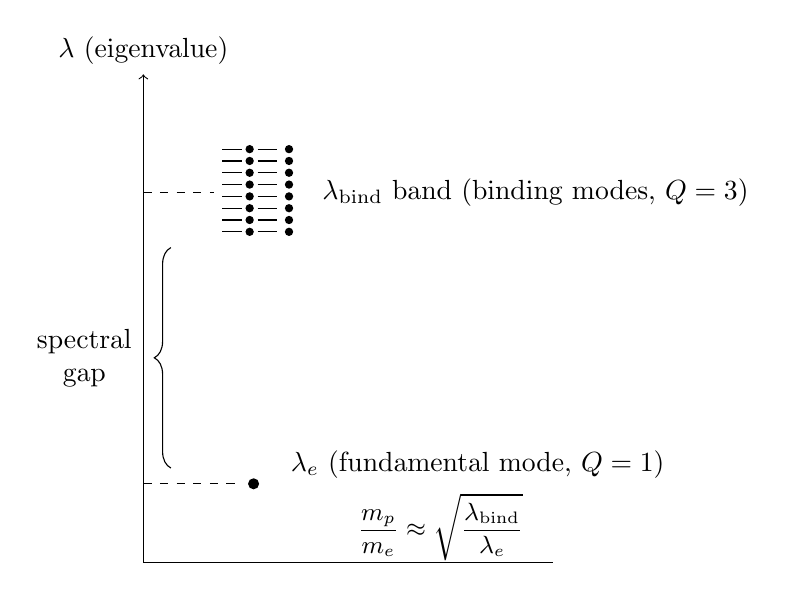
\begin{tikzpicture}[x=1cm,y=1cm]
      % Axis
      \draw[->] (0,0) -- (0,6.2) node[above] {$\lambda$ (eigenvalue)};
      \draw (0,0) -- (5.2,0);

      % Electron fundamental mode lambda_e
      \fill (1.4,1.0) circle (2pt);
      \node[anchor=west] at (1.75,1.25) {$\lambda_e$ (fundamental mode, $Q=1$)};

      % Binding band near lambda_bind
      \foreach \y in {4.2,4.35,4.5,4.65,4.8,4.95,5.1,5.25} {
        \draw (1.0,\y) -- (1.25,\y);
        \fill (1.35,\y) circle (1.5pt);
        \draw (1.45,\y) -- (1.70,\y);
        \fill (1.85,\y) circle (1.5pt);
      }
      \node[anchor=west] at (2.15,4.7) {$\lambda_{\mathrm{bind}}$ band (binding modes, $Q=3$)};

      % Indicate the gap with a brace
      \draw[decorate,decoration={brace,amplitude=6pt}]
      (0.35,1.2) -- (0.35,4.0)
      node[midway,xshift=-1.1cm,align=center] {spectral\\gap};

      % Optional dashed guide lines
      \draw[dashed] (0,1.0) -- (1.2,1.0);
      \draw[dashed] (0,4.7) -- (0.9,4.7);

      % Formula moved to the bottom-right (no overlap)
      \node[anchor=west,align=left] at (2.6,0.45)
        {\small $\displaystyle \frac{m_p}{m_e}\approx \sqrt{\frac{\lambda_{\mathrm{bind}}}{\lambda_e}}$};
    \end{tikzpicture}



\subsubsection{Summary and Outlook}

  Within the Cosmochrony framework, the proton-to-electron mass ratio is interpreted
  as an emergent constraint on the spectral and topological organization of solitonic
  excitations, not as a fundamental input parameter.

  The analysis presented here provides a coherent toy model identifying the
  conditions under which such a ratio could arise.
  Whether the required spectral hierarchy can be generated dynamically from the
  \(\chi\) relaxation dynamics remains an open problem, to be addressed through
  future analytical and numerical investigations.
